\documentclass[../main.tex]{subfiles}

\graphicspath{{\subfix{../figures/}}}

\begin{document}

\gls{cryoem} is an image acquisition technique that uses \glspl{tem} to examine a frozen sample. Unlike traditional optical microscopes, \glspl{tem} use an electron beam instead of light, which allows them to capture images at much higher resolution. As a consequence, it has become a very popular technique for collecting images of biological molecules, such as proteins\cite{chemistry_world_cryoem}. These images can be used to elucidate the 3D structure of the molecule under study.

However, \glspl{tem} require very specific conditions in order to work, such as near perfect vacuum and high-energy electrons. Therefore, they are unsuitable for biological samples, as these are too fragile to endure in such conditions. Here is where the cryogenic part comes into place. In order to retain the sample intact and in place, a thin film of ice is used. The sample is cooled down very rapidly, so that the water has no time to form an ice lattice, avoiding the diffraction of the electron beam. This technique was awarded with the 2017 Nobel Prize in Chemistry\cite{chemistry_world_cryoem}\cite{nobel2017}. Closely related to this, in 1982 Aaron Klug was also awarded with the Nobel Prize in Chemistry for his development of crystallographic methods to elucidate the 3D structure of proteins\cite{nobel1982}.

%\begin{figure}[htbp]
%    \centering
%    \begin{subfigure}[b]{0.3\textwidth}
%         \centering
%         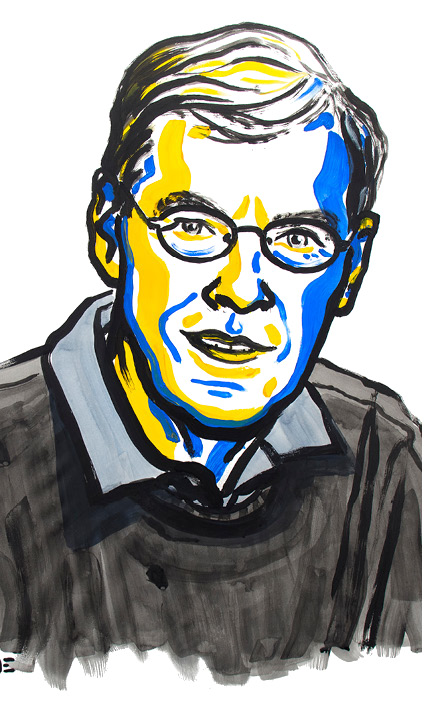
\includegraphics[width=\textwidth]{nobel2017/Richard Henderson}
%         \caption{Richard Henderson}
%         \label{fig:1:nobel2017:richard}
%    \end{subfigure}
%    \hfill
%    \begin{subfigure}[b]{0.3\textwidth}
%         \centering
%         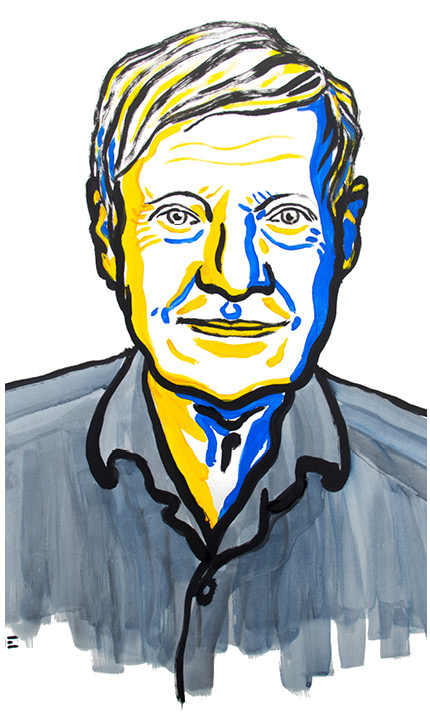
\includegraphics[width=\textwidth]{nobel2017/Joachim Frank}
%         \caption{Joachim Frank}
%         \label{fig:1:nobel2017:joachim}
%    \end{subfigure}
%    \hfill
%    \begin{subfigure}[b]{0.3\textwidth}
%         \centering
%         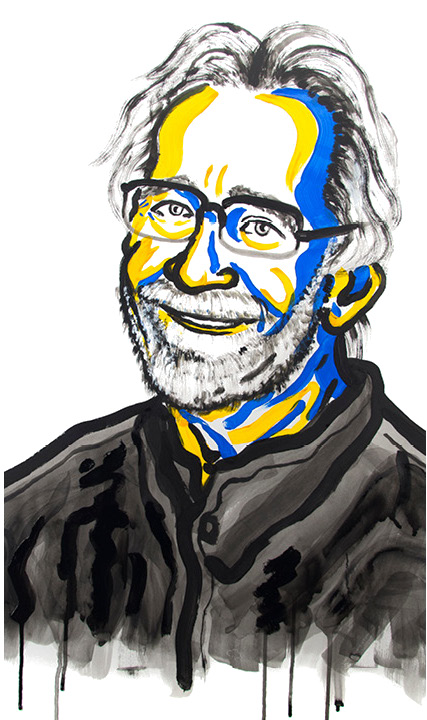
\includegraphics[width=\textwidth]{nobel2017/Jacques Dubochet}
%         \caption{Jacques Dubochet}
%         \label{fig:1:nobel2017:jaques}
%    \end{subfigure}\\
%    Images obtained from: \cite{science_nobel}
%    \caption{2017 Nobel Prize in Chemistry}
%    \label{fig:1:nobel2017}
%\end{figure}

Usually, the sample is prepared on a copper or gold grid, which may hold thousands of specimens under study, each of them with a random orientation. Each of these specimens is known as ``particle''. Assuming that all particles belong to the same structure, their 2D projections can be used to mathematically infer the 3D structure of the specimen\cite{cryoem101}. \Gls{spa} is a family of image acquisition and processing techniques that enables such a task.

At the beginning of the \gls{spa} image processing pipeline, a large quantity of noisy data is provided, from which little to no parameters are known. Therefore, all of the parameters needed for reconstruction must be estimated from the data. Many of these parameter estimations are conducted by assigning each experimental image to a reference image from which the parameters to be estimated are known. Thus, the parameters can be inherited from the assigned reference. This process is known as image alignment and it is one of the most frequent problems on a typical \gls{cryoem} image processing pipeline.

The aim of this project is to develop a fast computer program to align particles. The key innovation of this project is the usage of state-of-the-art vector search databases, which employ vector compression to store and compare vectors. 

The project has been carried out at the \gls{bcu} research group located at \gls{cnb}-\gls{csic} facilities. This research group develops two software suites related to \gls{cryoem}, Xmipp and Scipion. The former one implements image processing algorithms, whilst the later one provides a framework to easily interoperate between state-of-the-art image processing suites. Consequently, the software developed in this project will be implemented inside Xmipp and it will be integrated into Scipion.

\section{Objectives}
\subfile{1.1-Objectives}

\section{Structure of the document}
\subfile{1.2-Structure}

\end{document}
 